\everymath{\displaystyle}
\documentclass{beamer}
% \documentclass[handout]{beamer}

%\usepackage[pdftex]{color,graphicx}
\usepackage{amsmath,amssymb,amsfonts}

\mode<presentation>
{
  % \usetheme{Darmstadt}
  % \usetheme[hideothersubsections]{Hannover}
  % \usetheme[hideothersubsections]{Goettingen}
  \usetheme[hideothersubsections, right]{Berkeley}

  \usecolortheme{seahorse}
  % \usecolortheme{dolphin}
  \usecolortheme{rose}
  % \usecolortheme{orchid}

  \useinnertheme[shadow]{rounded}

  \setbeamercovered{transparent}
  % or whatever (possibly just delete it)
}

\mode<handout>{
  \setbeamercolor{background canvas}{bg=black!5}
  \usepackage{pgfpages}
  \pgfpagesuselayout{4 on 1}[a4paper,border shrink=5mm, landscape]
}

\usepackage[brazilian]{babel}
% or whatever

% \usepackage[latin1]{inputenc}
\usepackage[utf8]{inputenc}
% or whatever

\usepackage{times}
%\usepackage[T1]{fontenc}
% Or whatever. Note that the encoding and the font should match. If T1
% does not look nice, try deleting the line with the fontenc.


\title%[] % (optional, use only with long paper titles)
{Intervalos de Confiança de proporções}

\subtitle
{Incertezas de dados categóricos} % (optional)

\author%[] % (optional, use only with lots of authors)
{Felipe Figueiredo}% \and S.~Another\inst{2}}
% - Use the \inst{?} command only if the authors have different
%   affiliation.

\institute[] % (optional, but mostly needed)
{
}
  % \inst{1}%
  % Department of Computer Science\\
  % University of Somewhere
  % \and
  % \inst{2}%
  % Department of Theoretical Philosophy\\
  % University of Elsewhere}
% - Use the \inst command only if there are several affiliations.
% - Keep it simple, no one is interested in your street address.

\date%[] % (optional)
{}

% \subject{Talks}
% This is only inserted into the PDF information catalog. Can be left
% out. 



% If you have a file called "university-logo-filename.xxx", where xxx
% is a graphic format that can be processed by latex or pdflatex,
% resp., then you can add a logo as follows:

\pgfdeclareimage[height=1.6cm]{university-logo}{../logo}
\logo{\pgfuseimage{university-logo}}



% Delete this, if you do not want the table of contents to pop up at
% the beginning of each subsection:
\AtBeginSubsection[]
%\AtBeginSection[]
{
  \begin{frame}<beamer>{Sumário}
    \tableofcontents[currentsection,currentsubsection]
  \end{frame}
}


% If you wish to uncover everything in a step-wise fashion, uncomment
% the following command: 

% \beamerdefaultoverlayspecification{<+->}


\begin{document}

\begin{frame}
  \titlepage
\end{frame}

\begin{frame}{Sumário}
  \tableofcontents
  % You might wish to add the option [pausesections]
\end{frame}


%% Template
% \section{}

% \subsection{}

% \begin{frame}{}
%   \begin{itemize}
%   \item 
%   \end{itemize}
% \end{frame}

% \begin{frame}
%   \begin{columns}
%     \begin{column}{5cm}
%     \end{column}
%     \begin{column}{5cm}
%     \end{column}
%   \end{columns}
% \end{frame}

% \begin{frame}{}
%   \includegraphics[height=0.4\textheight]{file1}
%   \includegraphics[height=0.4\textheight]{file2}
%   \includegraphics[height=0.4\textheight]{file3}
%   \begin{figure}
%     \caption{}
%   \end{figure}
% \end{frame}

% \begin{frame}{}
%   \begin{definition}
%   \end{definition}
%   \begin{example}
%   \end{example}
%   \begin{block}{Exercício}
%   \end{block}
% \end{frame}

\section{Intervalo de confiança de uma proporção}

\subsection{Proporções x mensurações}

\begin{frame}{Amostras e populações}
  \begin{block}{Estudos clínicos}
    \begin{itemize}
    \item a amostra de pacientes do estudo raramente é representativa da população global...
    \item ... mas pode ser representativa de uma população de pacientes semelhantes
    \end{itemize}
  \end{block}
  \begin{block}{Experimentos de laboratório}
    \begin{itemize}
    \item Geralmente difícil de definir
    \item Reprodução de experimentos semelhantes
    \end{itemize}
  \end{block}
\hfill Cap. 1
\end{frame}

\begin{frame}{Proporções x mensurações}
  % \begin{block}{Definição}
  %   Mensuração é a atribuição de um número a uma característica de um objeto ou evento, que por sua vez pode ser comparada com outros objetos ou eventos.
  % \end{block}
  \begin{itemize}
  \item Resultados de experimentos podem ser expressos de várias maneiras
  \item As duas principais são a mensuração e a proporção
  \end{itemize}
  \begin{exampleblock}{Exemplo}
    \begin{itemize}
    \item prop. de pacientes com infecção após um procedimento
    \item prop. de estudantes aprovados em um curso (de Bioestatística)
    \end{itemize}
  \end{exampleblock}
\end{frame}

\subsection{Da população para a amostra}

\begin{frame}{A distribuição Binomial}
  \begin{itemize}
  \item Ao jogar uma moeda:
    \begin{itemize}
    \item 50\% de dar cara
    \item 50\% de dar coroa
    \end{itemize}
  \item Se \alert{você} jogar uma moeda  algumas vezes:
    \begin{itemize}
    \item você vai tirar cara {\em exatamente} 50\% das vezes?
    \item Por que?
    \end{itemize}
  \end{itemize}
\end{frame}

\begin{frame}{A distribuição Binomial}
  \begin{exampleblock}{Exemplo}
    Qual é a proporção de meninas entre 14 neonatos?
  \end{exampleblock}
  \begin{block}{Pense...}<2->
    \begin{itemize}
    \item Esse grupo de neonatos é uma amostra ou uma população?
    \item<3-> Qual é a população?
    \item<4-> Essa amostra \alert{representa} a população?
    \item<5
      -> Se você observar {\em vários} grupos de 14 neonatos... quantas meninas devem nascer em cada amostra?
    \end{itemize}
  \end{block}

\end{frame}

\begin{frame}{A distribuição Binomial}
  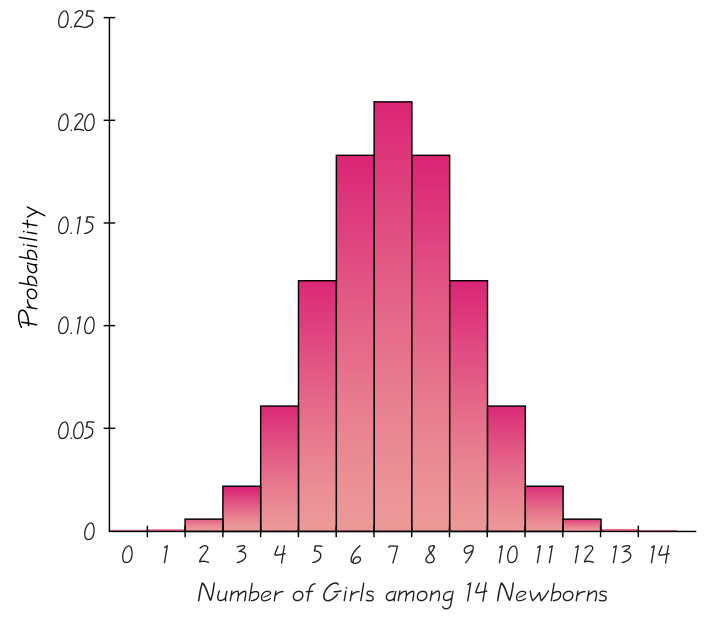
\includegraphics[height=\textheight]{Prob_II/discreta}
\end{frame}


\begin{frame}{A distribuição Binomial}
  \begin{block}{}
    Amostras de populações com proporções diferentes
  \end{block}

  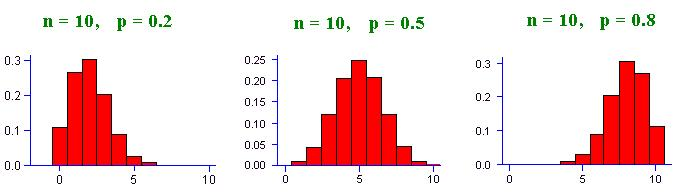
\includegraphics[width=\textwidth]{Prob_II/binomial}
\end{frame}

\subsection{Da amostra para a população}

\begin{frame}{O Intervalo de Confiança de uma proporção}
  \begin{exampleblock}{Exemplo}
    De cada 14 pacientes tratados com um certo medicamento, 3 sofreram um evento adverso.

    A proporção é $\frac{3}{14} = 0.2143$.
  \end{exampleblock}
  \begin{block}{Pense...}<2->
    \begin{itemize}
    \item Esta amostra representa toda a população de pacientes que receberá este medicamento?
    \item<3-> Isto é... Quais foram os critérios de inclusão?
    \item<4-> A proporção desta amostra reflete a proporção da população?
    \end{itemize}
  \end{block}

\end{frame}

\begin{frame}{O Intervalo de Confiança de uma proporção}
    \begin{exampleblock}{Exemplo}
    Uma pesquisa de boca de urna entrevistou 100 pessoas, e apenas 33 declararam intenção de voto no canditado A.

    % A proporção é $\frac{33}{100} = $.
  \end{exampleblock}
  \begin{block}{}<2->
    \begin{itemize}
    \item Esta amostra representa a população de eleitores?
    \item<3-> Os entrevistados falaram a verdade sobre em quem votarão?
    \item<4-> Assumindo representatividade...
    \item<4-> Os entrevistados representam a mesma proporção da população?
    \end{itemize}
  \end{block}
\end{frame}

\begin{frame}{O Intervalo de Confiança de uma proporção}
  \begin{itemize}
  \item Sabendo a prop. da amostra, não há como garantir que sabemos a prop. da população
  \item Plano B: calcular um intervalo onde {\em acreditamos} que a prop. da população está.
  \item P: Qual deveria ser o tamanho deste intervalo?
  \end{itemize}
\end{frame}

\begin{frame}{O Intervalo de Confiança de uma proporção}
  \begin{itemize}
  \item Se o intervalo for muito grande: a prop. da população deve estar contido
  \item Se o intervalo for muito pequeno: a prop. da população pode não estar
  \item {\bf P: Como saber?}
  \end{itemize}
\end{frame}

\begin{frame}{O Intervalo de Confiança de uma proporção}
  \begin{itemize}
  \item {\bf P: Como saber?}
  \item R: Geralmente aceitamos 5\% de que a prop. da população não está no intervalo criado
  \item Ou seja: temos \alert{95\% de confiança} de que o intervalo cumpriu seu papel
  \end{itemize}
\end{frame}

\begin{frame}{O Intervalo de Confiança de uma proporção}
  \begin{exampleblock}{Exemplo}
    De cada 14 pacientes tratados com um certo medicamento, 3 sofreram um evento adverso.

    A proporção é $\frac{3}{14} = 0.2143$.
  \end{exampleblock}
    \begin{exampleblock}{Exemplo}
    Uma pesquisa de boca de urna entrevistou 100 pessoas, e apenas 33 declararam intenção de voto no canditado A.

    % A proporção é $\frac{33}{100} = $.
  \end{exampleblock}
  \begin{itemize}
    \item Tente {\em imaginar} um intervalo que \alert{provavelmente contém} a proporção desejada para estes exemplos
    \item (e anote num papel)
  \end{itemize}
\end{frame}

\begin{frame}{O Intervalo de Confiança de uma proporção}
  \begin{itemize}
  \item Intuição: intervalos menores que o intervalo correto
  \item O \alert{Intervalo de Confiança} (IC) do primeiro exemplo é: [5\%, 51\%]
  \item O IC do segundo exemplo é: [24\%, 42\%]
  \item<2-> Note os tamanhos dos dois ICs
  \end{itemize}
\end{frame}


\subsection{"95\% de confiança"?}

\begin{frame}{"95\% de confiança"?}
  \begin{itemize}
  \item Softwares: fácil calcular o IC de uma amostra
  \item Mas temos apenas \alert{uma} amostra
  \item E se obtivéssemos outra amostra?
  \end{itemize}
\end{frame}

\subsection{Premissas}

\begin{frame}{Premissas}
  \begin{itemize}
  \item Amostra aleatória / amostra representativa
  \item Observações independentes
  \item Avaliações corretas
  \item Avaliar um evento {\bf relevante}
  \end{itemize}
\end{frame}

\subsection{Exercício(s)}

\begin{frame}{Exercício (cap 2)}
  \begin{block}{Exercício 1}
    Dos 100 primeiros pacientes que passam por uma cirurgia, 6 morreram.
    Você pode calcular o IC da probabilidade de morrer neste procedimento?

    Caso sim, Encontre o IC (já tenho a cola).

    Caso não, que outras informações você precisa?

    Que hipóteses você precisa fazer?
  \end{block}
\end{frame}

\begin{frame}{Leitura pós-aula e exercícios selecionados}
  \begin{block}{Leitura obrigatória}
    Capítulo 2.

    Pular as seções
    \begin{itemize}
    \item Tabelas de ICs
    \item casos especiais 0\% e 100\%
    \item cálculo do IC
    \item Equação binomial
    \item Como os ICs são derivados
    \end{itemize}

  \end{block}
  \begin{itemize}
  \item Exercício 1 (caso precise do IC: [2\%, 13\%])
  \item Exercício 2 (caso precise do IC: [2\%, 13\%])
  \item Exercício 4 (caso precise do IC: [10\%, 24\%])
  \end{itemize}
\end{frame}

\end{document}
